\setcounter{chapter}{11}
\chapter{Профилирование и анализ производительности кода}
Предыдущая лекция была посвящена тестам. Если представить, что программное обеспечение --- это корабль, то тесты позволяют убедиться в том, что большая часть этого корабля не обладает дырками, не протекает, работает правильно. Но это совершенно не означает, что он будет плавать. Корабль может быть настолько тяжелый, что он сразу пойдет ко дну.

Поэтому вторая вещь, на которую нужно проверять программное обеспечение --- это производительность.

\section{Профилирование}
Профилирование --- сбор характеристик работы программы, таких как время выполнения отдельных фрагментов или потребления иных ресурсов. Профилирование проводится с целью поиска возможности оптимизации потребления этих ресурсов.


\subsection{Ресурс процессора}
Когда речь идет о процессоре, всегда встает вопрос --- измерять время процессора (cpu time) или реальное время.

Когда измеряется cpu time, измеряется именно время, которое было потрачено на конкретное приложение. Однако таймер, который считает потребленное время процессора, имеет довольно низкую точность. Также это время не включает в себя ожидание ввода-вывода. Программа, которая считывает что-либо из файла или записывает в файл, реальное время исполнения будет значительно больше потребленного процессорного времени.

Поэтому при оценке времени исполнения программы лучше ориентироваться на реальное время. Оно может быть очень точно измерено и включает в себя время ожидания ввода-вывода. Однако реальное время исполнения сильно зависит от загрузки системы.

\subsection{Измерение реального и процессорного времени}
Консольная утилита time позволяет измерить, сколько прошло реального времени и сколько было потреблено процессорного времени.

В качестве тестовой программы будет использоваться скрипт, загружающий веб-страницу.
\begin{minted}{bash}
$ time perl -MLWP::UserAgent -E \
'LWP::UserAgent->new->get("https://mail.ru/");'
\end{minted}

Результаты измерения утилитой time:
\begin{verbatim}
real    0m0.056s
user    0m0.043s
sys     0m0.008s
\end{verbatim}
Можно ли считать, что все указанное время было потрачено на запрос? Чтобы выяснить это, можно слегка модифицировать скрипт и выполнить 100 запросов вместо одного:

\begin{minted}{bash}
$ time perl -MLWP::UserAgent -E \
'LWP::UserAgent->new->get("https://mail.ru/")
 for 1..100;'
\end{minted}

Результаты измерений оказываются следующими:
\begin{verbatim}
real    0m0.164s
user    0m0.104s
sys     0m0.022s
\end{verbatim}
Если считать, что все время тратится только на запросы, то проведенные два измерения не согласуются друг с другом.

\subsection{Профилирование в perl}
На данный момент лучшим профилировщиком является так называемый \verb|Devel::NYTProf| (New York Times Profiler). Команда New York Times взяли в качестве основы \verb|Devel::Prof| и стали дорабатывать его.

\verb|Devel::NYTProf| должен быть подключен в режиме дебаггера:
\begin{minted}{bash}
$ perl -d:NYTProf -MLWP::UserAgent -E \
'LWP::UserAgent->new->get("https://mail.ru/")
 for 1..100;'
\end{minted}
Здесь ключ \verb|-d| обозначает запуск дебаггера. В результате этой команды появляется файл \verb|nytprof.out|, собственно профиль.
\begin{minted}{bash}
$ ls -la *out
\end{minted}
\begin{verbatim}
-rw-r--r-- 1   mons staff 314206   nytprof.out
\end{verbatim}
Этот файл можно легко превратить в различного рода диаграммы, схемы, страницы и так далее. nytprofhtml конвертирует этот файл в директорию nytprof, где будет лежать html-страница и все сопутствующие файлы.
\begin{minted}{bash}
$ nytprofhtml
\end{minted}

\begin{minted}{bash}
$ ls -lad nytprof
\end{minted}
\begin{verbatim}
drwxr-xr-x 200 mons staff 6800     nytprof
\end{verbatim}
Например, итоговая страница может выглядеть вот так:
\begin{figure}[H] % Картинка
	\centering
	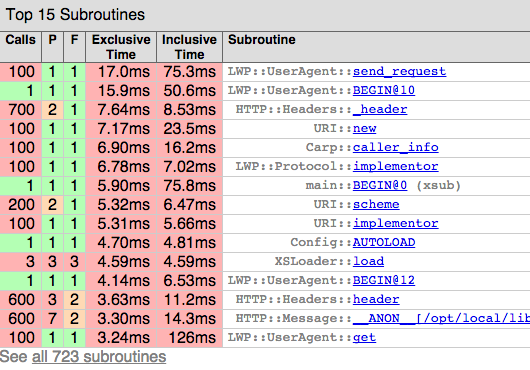
\includegraphics[width=10cm]{lectures/L12/nyt1.png}
\end{figure}


Профайлер замерил время выполнения всех функций, сколько раз они запускались и так далее. Функции отсортированы по времени исполнения и по умолчанию показаны только 15 из них.

\subsection{Inclusive и exclusive время исполнения}
Разница между inclusive и exclusive временем следующая. Пусть выполняется некоторая функция \verb|foo()|, которая вызывает дважды функцию \verb|bar()|.
\begin{figure}[H] % Картинка
	\centering
	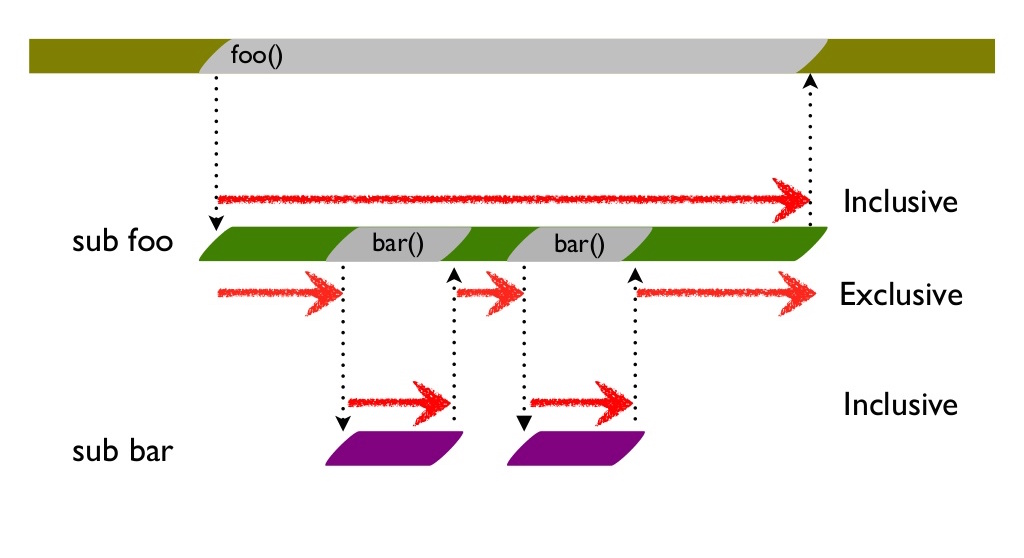
\includegraphics[width=10cm]{lectures/L12/inclusive-exclusive.jpg}
\end{figure}
Тогда inclusive time --- это время от входа в функцию до выхода из функции \verb|foo()|. Пока функция \verb|foo()| исполнялась, она исполняла другие функции. Соответственно время, которое было потрачено непосредственно на sub foo за вычетом вызовов других функций называется exclusive time. Практическим следствием отсюда является тот факт, что если у некоторой функции iclusive time большой, а exclusive time --- значительно меньше, то тормозит не она, а какая-то еще функция, которую она вызывает.

\subsection{Режим start=init}
От функций, которые исполняются один раз, в профиле можно избавиться, запустив профилировщик в режиме \verb|start=init|:
\begin{verbatim}
$ NYTPROF=start=init \
  perl -d:NYTProf -MLWP::UserAgent -E \
 'LWP::UserAgent->new->get("https://mail.ru/")
 for 1..100;'
$ nytprofhtml
\end{verbatim}
Здесь флаг \verb|start| задает момент, когда нужно запустить профилировщик. В данном случае он запускается после того, как выполнены все \verb|use|'ы, \verb|BEGIN|'ы и так далее. В результате получаются следующие результаты измерений:
\begin{figure}[H] % Картинка
	\centering
	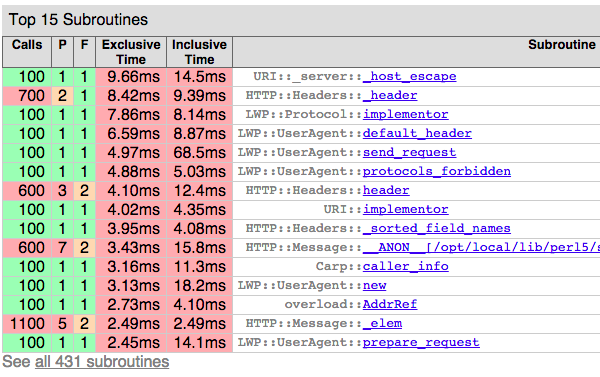
\includegraphics[width=10cm]{lectures/L12/nyt2.png}
\end{figure}

\subsection{Режим start=no}
В режиме \verb|start=no| профилировщик не запускается сам. После того, как все будет подготовлено, он будет запущен с помощью модуля \verb|DB|. Модуль \verb|DB| позволяет управлять дебаггером, в частности включать и выключать профилирование.

В данном конкретном случае не важно, сколько времени занимает загрузка модулей и создание объекта, а важно, чтобы определенный участок работал быстро:
\begin{verbatim}
$ NYTPROF=start=no \
  perl -d:NYTProf -MLWP::UserAgent -E \
 'my $ua = LWP::UserAgent->new;
  DB::enable_profile();
  $ua->get("https://mail.ru/") for 1..100;
  DB::disable_profile();'
$ nytprofhtml
\end{verbatim}
\begin{figure}[H] % Картинка
	\centering
	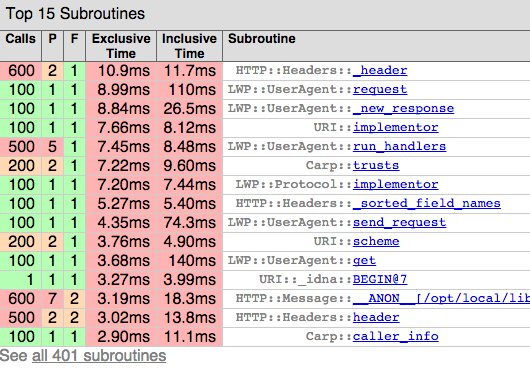
\includegraphics[width=10cm]{lectures/L12/nyt3.png}
\end{figure}
Теперь в профиле не содержится создание объекта и <<в топ вылезли>> функции \verb|_header| и \verb|request|. 
\begin{figure}[H] % Картинка
	\centering
	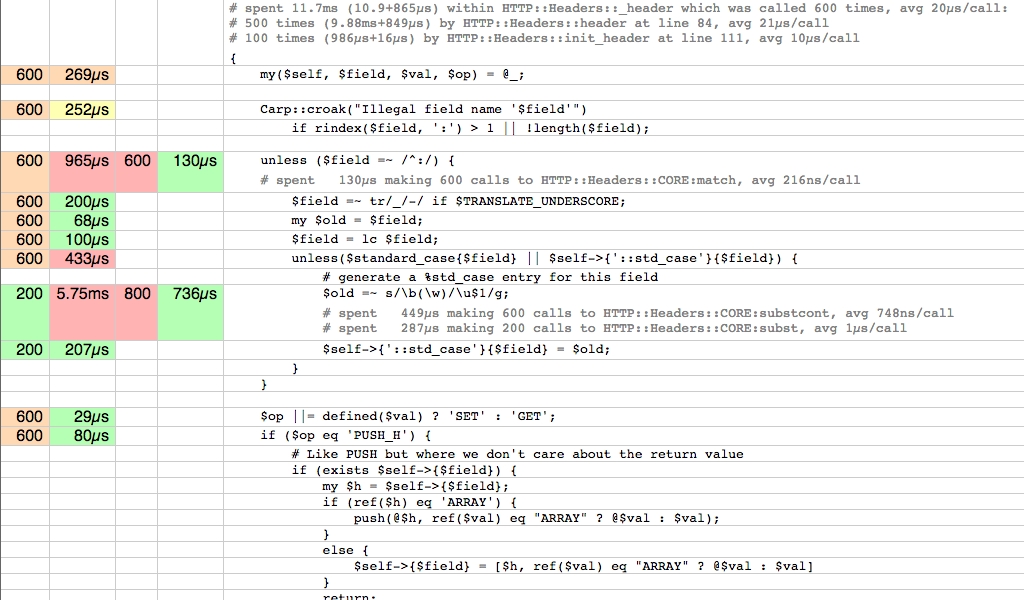
\includegraphics[width=13cm]{lectures/L12/nyt4.png}
\end{figure}
Причем inclusive time у функции \verb|request| значительно больше exclusive time. Эта разница обусловлено временем ожидания ввода-вывода в функции request.

\subsection{Flame Graph}
Flame Graph позволяет визуально увидеть, на что идет потраченное время.
\begin{figure}[H] % Flame Graph
	\centering
	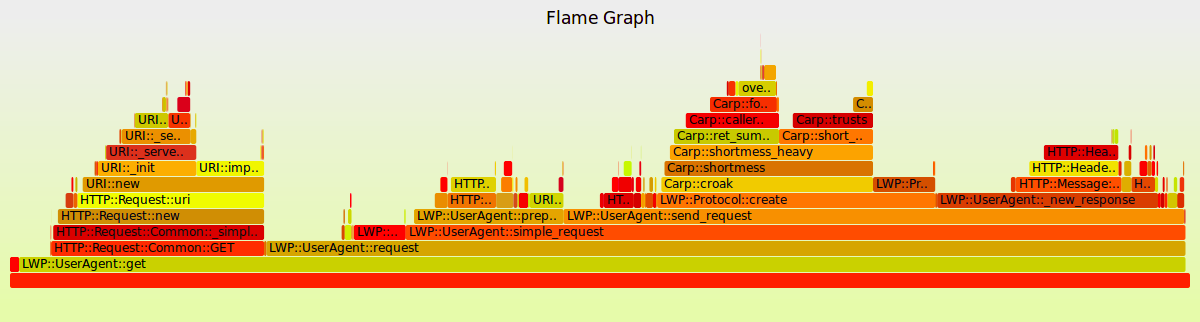
\includegraphics[width=15cm]{lectures/L12/flame.png}
\end{figure}
На этой картинке изображено суммарное время исполнения программы и по частям на что оно ушло. Причем на каждую вещь можно кликать и смотреть, из чего она состояла. Можно посмотреть, сколько раз вызывалась конкретная функция и сколько времени занимало исполнение конкретных строк.
\begin{figure}[H]
\end{figure}
\verb|NYTProf| пишет, сколько времени он провел внутри этой функции, сколько раз она вызывалась, какое среднее время исполнения функции, а также кто ее вызывал:
\begin{verbatim}
spent 11.7ms (10.9+865µs) within
    HTTP::Headers::_header which was called
    600 times, avg 20µs/call:
    500 times (9.88ms+849µs)
        by HTTP::Headers::header at line 84,
        avg 21µs/call
    100 times (986µs+16µs)
        by HTTP::Headers::init_header at line 111,
        avg 10µs/call
\end{verbatim}
Также под каждую строчку он пишет, сколько времени он проводил в конкретных вызовах. Вызов regexp'ов присутствует в виде функций \verb|CORE:match|, \verb|CORE:substcont| и \verb|CORE:subst|.
\begin{minted}{perl}
unless ($field =~ /^:/)
    # spent   130µs making 600 calls to
    HTTP::Headers::CORE:match, avg 216ns/call

$old =~ s/\b(\w)/\u$1/g;
    # spent   449µs making 600 calls to
        HTTP::Headers::CORE:substcont,
        avg 748ns/call
    # spent   287µs making 200 calls to
        HTTP::Headers::CORE:subst,
        avg 1µs/call
\end{minted}


\section{Оптимизация}
\subsection{Правила оптимизации}
Первое правило оптимизации --- не оптимизируйте программы. Второе правило оптимизации программ --- не оптимизируйте программы, пока это не понадобится. Большая часть проблем в софте возникает из-за того, что кто-то начинает оптимизировать программы раньше, чем это реально понадобилось. К этим проблемам относятся:
\begin{itemize}
  \item Превращение программы в нечитаемый код
  \item Программа превращается в огромный код
  \item Программу становится сложно поддерживать
  \item Делается ошибочное допущение без проверки
\end{itemize}

\subsection{Порядок профилирования и оптимизации программы}
Tim Bunce описал правила, как правильно профилировать программу:
\begin{enumerate}
    \item Даём репрезентативную нагрузку
      Репрезентативной нагрузкой называется нагрузка, которая соответствует тому окружению, в котором будет работать ваше приложение.
    \item Смотрим общее время функций
      Нужно адекватно оценивать возможности железа и perl при оценке времени.
    \item Время выглядит адекватно?
      Должна ли программа должна работать во много раз быстрее?
    \item Исследуем самые медленные участки
      Для этого необходимо профилировать в разных режимах.
    \item Исправляем простые проблемы
      Сначала необходимо найти простые ошибки (по невнимательности или из-за простоты написания) и оптимизировать их.
    \item Профилируем заново
    \item Производительность хорошая? СТОП!
    \item Повторите 1-2 раза
    \item Переходите к другим улучшениям.
\end{enumerate}

\subsection{Пример оптимизации}
Пусть дана строка из 1024 символов и две функции, которые вырезают первые 10 символов строки разными способами:
\begin{minted}{perl}
    my $str = "x"x1024;

    sub func1 {
      my $s = $str;
      substr($s,0,10,"");
    }

    sub func2 {
      my $s = $str;
      $s = substr($s,10);
    }
\end{minted}


Какая из двух функций будет работать быстрее? Из-за того, что 10 --- величина очень маленькая, и в perl действует хитрая оптимизация, которая позволяет смещать начало строки без реаллокации, функция \verb|func1| скорее всего будет работать быстрее. Но чтобы убедиться в этом, это нужно проверить. Также всегда нужно проверять скорость работы именно для тех данных и для того окружения и железа, которые будут в реальной работе.

\subsection{Модуль Benchmark}
Один из способов проверить --- использовать модуль \verb|Benchmark|. Если в качестве первого параметра подается положительное число, функция исполняется именно такое число раз. Если подано отрицательное значение, функция будет исполняться до тех пор, пока затраченное процессорное время не будет равно модулю этого значения.
\begin{minted}{perl}
  use Benchmark qw(:all);
  timethis(1e6,\&func1);
  timethis(-1,\&func1);
\end{minted}
Результат выполнения следующий:
\begin{verbatim}
timethis 1000000:  0 wallclock secs
    ( 0.20 usr +  0.01 sys =  0.21 CPU)
        @ 4761904.76/s (n=1000000)
(warning: too few iterations for a reliable count)
timethis for 1:  1 wallclock secs
    ( 1.02 usr +  0.00 sys =  1.02 CPU)
        @ 4665608.82/s (n=4758921)
\end{verbatim}
Помимо простого измерения модуль \verb|Benchmark| позволяет сравнивать между собой различные функции:
\begin{minted}{perl}
use Benchmark qw(:all);
timethese -1, {
    inplace => \&func1,
    copy    => \&func2,
};
\end{minted}
Результат выполнения следующий:
\begin{verbatim}
Benchmark: running copy, inplace for
    at least 1 CPU seconds...
copy:  2 wallclock secs
    ( 1.00 usr +  0.02 sys =  1.02 CPU)
        @ 4151600.98/s (n=4234633)
inplace:  1 wallclock secs
    ( 1.09 usr +  0.01 sys =  1.10 CPU)
        @ 4549606.36/s (n=5004567)
\end{verbatim}

\subsection{Модуль Dumbbench}
Модуль \verb|Dumbbench| позволяет выполнить серию начальных запусков.
\begin{minted}{perl}
use Dumbbench;
my $bench = Dumbbench->new(
    target_rel_precision => 0.005,
    initial_runs         => 50,
);
$bench->add_instances(
    Dumbbench::Instance::PerlSub
      ->new(name => 'inplace', code => \&func1),
    Dumbbench::Instance::PerlSub
      ->new(name => 'copy', code => \&func2),
);
$bench->run();
$bench->report();
\end{minted}
Результат выполнения следующий:
\begin{verbatim}
inplace: Ran 93 iterations (26 outliers).
inplace: Rounded run time per iteration:
    1.5462e-07 +/- 3.4e-10 (0.2%)
copy: Ran 56 iterations (6 outliers).
copy: Rounded run time per iteration:
    4.0881e-07 +/- 6.0e-10 (0.1%)
\end{verbatim}

\subsection{/dev/hands}
Помимо использования готовых модулей и утилит, можно реализовать процесс профилирования вручную. В perl есть функция \verb|times|, которая возвращает текущее потребление user time и system time. Тогда код будет иметь вид:
\begin{minted}{perl}
use List::Util qw(sum); my $N = 4e6;
my $cpu = sum((times)[0,1]);
func1() for 1..$N;
my $cpu1 = sum((times)[0,1]);
printf "%0.3fs CPU, %0.1fns/call\n",
$cpu1-$cpu, (1e9/$N)*($cpu1-$cpu);
func2() for 1..$N;
my $cpu2 = sum((times)[0,1]);
printf "%0.3fs CPU, %0.1fns/call\n",
$cpu2-$cpu1, (1e9/$N)*($cpu2-$cpu1);
\end{minted}
Результат выполнения следующий:
\begin{verbatim}
1.320s CPU, 330.0ns/call
1.460s CPU, 365.0ns/call
\end{verbatim}

\section{Оптимизация: Простые локальные изменения}

\begin{itemize}
\item Вынести постоянные выражения за пределы цикла
\begin{minted}{perl}
for (...) {
	my $a = 123;
	call_sub($a);
}

my $a = 123;
for (...) {
	call_sub($a);
}
\end{minted}
	\item Избегать повторения цепочек аксессоров
Следующий код:
\begin{minted}{perl}
Avoid->repeated()->chains()->of->accessors();
Avoid->repeated()->chains()->of->accessors();
Avoid->repeated()->chains()->of->accessors();
\end{minted}
можно оптимизировать введя новую переменную:
\begin{minted}{perl}
my $one = Avoid->repeated()->chains()->of;
$one->accessors();
$one->accessors();
$one->accessors();
\end{minted}
\item Не вызывайте те функции, которые можно не вызывать:
\begin{minted}{perl}
use constant DEBUG => 0;
my $unused = $self->get_something;
my $do_log = $logger->logging;
for (...) {
	$logger->log(...) if $do_log;
	do_debug(...) if DEBUG;
	...
}
\end{minted}

\item Выходите раньше, инициализируйте позже
\begin{minted}{perl}
sub {
    return unless @_;
    return 1 if @_ == 1;
    for (@_) { ... }
    ...
}
sub {
    if () { ... }
    elsif () { ... }
    else {
        return;
    }
}
\end{minted}

\item Избегайте ненужных проверок
\begin{minted}{perl}
- return exists $hash{$something}{$key}
-             ? $hash{$something}{$key}
-             : undef

+ return $hash{$something}{$key}
\end{minted}
\item Используйте аргументы без распаковки в наиболее часто вызываемых функциях
\begin{minted}{perl}
sub add ($$) {
    return $_[0] + $_[1]
}
\end{minted}

\item Внести цикл под вызов
\begin{minted}{perl}
$object->walk($_) for @dogs;
$object->walk_that(\@dogs);
\end{minted}
\end{itemize}


\section{Оптимизация: значительные изменения}
Попытайтесь найти быстрый модуль, чем тот, что используется сейчас. На сайте \url{http://neilb.org/reviews/} регулярно проводятся обзоры модулей и сравнивает их по потреблению ресурсов и по функционалу.

Еще один неочевидный способ повысить производительность --- обновить и/или пересобрать perl:
\begin{itemize}[nosep]
	\item Сборка без тредов дает до +30\%
	\item Сборка без отладки дает до +5\%
	\item 5.10 -> 5.16 может дать до +15\%
	\item 5.16 -> 5.20 может дать до +20\%
\end{itemize}


Оптимизация алгоритмов
\[    O(n^2) \to O(n \log n) \to O(n) \to O(\log n) \to O(1) \]

Переписывание <<горячих>> участков на XS

% TODO 1:37:32
\section{Память}
Второй ресурс, который становится критичен, это память. При создании небольших приложений потреблению памяти обычно не уделяется внимание. Если процесс должен обрабатывать большие объемы данных, вопрос потребления памяти становится особенно актуален.

Классический пример утечки памяти --- циклическая ссылка.
\begin{minted}{perl}
my $x;$x = \$x; # << selfref

my $h = {};
$h->{key} = $h; # << cyclic ref

my $s;$s = sub {
    $s->(); # << ref by closure
};
\end{minted}
При создании циклической ссылки сборщик мусора в perl уже не может уничтожить данную переменную автоматически. Это связано с тем, что переменная ссылается сама на себя и счетчик ссылок никогда не достигнет нуля.

Для обнаружения утечек используется модуль \verb|Devel::Leak|.
\begin{minted}{perl}
use Devel::Leak;
Devel::Leak::NoteSV($handle);

my $x;$x = \$x;
my $h = {};$h->{key} = $h;
my $s;$s = sub {$s->();};

Devel::Leak::CheckSV($handle);
\end{minted}
Сначала создается заметка, затем исполняется требуемый код и вызываеся проверка на этой заметке:
\begin{minted}{perl}
new 0x7fc84b021b28 :
new 0x7fc84b021b40 :
new 0x7fc84b021b58 :
new 0x7fc84b021b70 :
new 0x7fc84b021c00 :
new 0x7fc84b021c18 :
new 0x7fc84b004ce8 :
new 0x7fc84b004ec8 :
\end{minted}
Если perl собран с флагом -DDEBUGGING (то есть с отладкой), вывод будет более подробный:
\begin{minted}{bash}
new 0x2410de8 : SV = PVHV(0x2416e40) at 0x2410de8
  REFCNT = 2
  FLAGS = (SHAREKEYS)
  ARRAY = 0x24aa640  (0:7, 1:1)
  hash quality = 100.0%
  KEYS = 1
  FILL = 1
  MAX = 7
  RITER = -1
  EITER = 0x0
new 0x2410f68 : SV = IV(0x2410f58) at 0x2410f68
  REFCNT = 1
  FLAGS = (ROK)
  RV = 0x2410de8
    SV = PVHV(0x2416e40) at 0x2410de8
      REFCNT = 2
      FLAGS = (SHAREKEYS)
      ARRAY = 0x24aa640  (0:7, 1:1)
\end{minted}
По этой информации уже можно понять, что именно утекло.

Другой способ найти утечку памяти --- использовать переменную, в которой хранится число используемых SV:
\begin{minted}{perl}
int checkpoint = PL_sv_count;

/* ...some leaky code... */

printf("leaked by %d SV's",
    PL_sv_count - checkpoint);
\end{minted}
Если код при своем повторении не создает лишние SV, то есть все что он создал, он потом уничтожил, то будет выведен ноль.

При использовании Linux, утечку памяти можно обнаружить вручную:
\begin{minted}{bash}
/proc/[pid]/statm
  Provides information about memory usage.

  size   total program size
         (same as VmSize in /proc/[pid]/status)
  resident   resident set size
         (same as VmRSS in /proc/[pid]/status)
  share  shared pages (from shared mappings)
  text   text (code)
  lib    library (unused in Linux 2.6)
  data   data + stack
  dt     dirty pages (unused in Linux 2.6)
\end{minted}
Для этого удобно создать функцию mem:
\begin{minted}{perl}
use POSIX qw( _SC_PAGESIZE sysconf );
my $PG = sysconf(_SC_PAGESIZE);
sub mem () {
    open my $f,'<:raw','/proc/self/statm';
    my ($all,$rss,$shr,$txt,$lib,$data) =
    map $_*$PG, split /\s+/, scalar <$f>;
    return $data;
}

my $before = mem();
for (1..1e5) {
    my %h;$h{key} = \%h;
}
my $after = mem();
printf "Lost %0.1fM\n",
    ($after-$before)/1024/1024;
\end{minted}
В результате исполнения кода будет выведено количество потерянной памяти после прогона:
\begin{minted}{bash}
Lost 17.7M
\end{minted}
В связи с особенность выделения памяти в perl, не всегда увеличение используемой памяти значит утечку. В этом случае следует увеличить число итерации --- в случае утечки память будет расти линейно в зависимости от номера итерации.

Если используется не Linux, можно воспользоваться модулем Proc::ProcessTable:
\begin{minted}{perl}
use Proc::ProcessTable;
my $t = Proc::ProcessTable->new();

for my $p ( @{ $t->table } ) {
  next unless $$ == $p->pid;
  say $p->pid," ", $p->size;
}
\end{minted}
Если утечка памяти происходит в модуле XS:
\begin{minted}{c++}
void test(SV *var)
PPCODE:
    SV *leaky = newSVpvs("dummy");
    XSRETURN_UNDEF;
\end{minted}
После использования Devel::Leak:
\begin{minted}{perl}
use Devel::Leak;
Devel::Leak::NoteSV(my $chk);
LeakTest::test($smth);
Devel::Leak::CheckSV($chk);
\end{minted}
оказалось, что есть утечка:
\begin{minted}{bash}
new 0x1496a68 :
\end{minted}
В этом случае есть способ определять место утечки с помощью опорной переменной:
\begin{minted}{c++}
void test(SV *var)
PPCODE:
    SV *leaky = newSVpvs("dummy");
    printf("var = %p\n",var);
    SV * ghost = (SV *) ( (char *)var + 0 );
    sv_dump( ghost );
    XSRETURN_UNDEF;
\end{minted}
Таким образом, известен адрес опорной переменной и утекающей переменной.
\begin{minted}{bash}
var = `0x2075c38`
SV = NULL(0x0) at `0x2075c38`
  REFCNT = 1
  FLAGS = (PADMY)
new `0x2058a68` :
\end{minted}
Можно подсчитать разницу:
\begin{minted}{bash}
0x2058a68 - 0x2075c38 = -119248
\end{minted}
и подставить эту разницу обратно в код:
\begin{minted}{c++}
void test(SV *var)
PPCODE:
    SV *leaky = newSVpvs("dummy");
    printf("var = %p\n",var);
    SV * ghost = (SV *) ( (char *)var - `119248` );
    sv_dump( ghost );
    XSRETURN_UNDEF;
\end{minted}
Поскольку код не изменился (только изменилось число), адреса не сдвинутся. После запуска опорная переменная останется на том же месте, а также становится известна информация об утекшей переменной:
\begin{minted}{bash}
var = 0x20f2c38
SV = PV(0x20d3cf0) at `0x20d5a68`
  REFCNT = 1
  FLAGS = (POK,pPOK)
  PV = 0x21ab7a0 "dummy"\0
  CUR = 5
  LEN = 16
new `0x20d5a68` :
\end{minted}
Чтобы исправить утечку, необходимо добавить \verb|sv_2mortal|:
\begin{minted}{c}
void test(SV *var)
PPCODE:
    SV *leaky = sv_2mortal(newSVpvs("dummy"));
    printf("var = %p\n",var);
    SV * ghost = (SV *) ( (char *)var - `119248` );
    sv_dump( ghost );
    XSRETURN_UNDEF;
\end{minted}
\begin{minted}{bash}
var = 0x20f2c38
SV = PV(0x20d3cf0) at `0x20d5a68`
  REFCNT = 1
  FLAGS = (POK,pPOK)
  PV = 0x21ab7a0 "dummy"\0
  CUR = 5
  LEN = 16
\end{minted}


Self-referenced closure:
\begin{minted}{perl}
my $cb; $cb = sub {
    something_async sub {
        $cb->();
    };
};
$cb->();
\end{minted}
В perl есть возможность создавать слабые ссылки. То есть есть ссылка на какой-то блок, которая не удерживает +1 на счетчике ссылок. Not very self-referenced closure:
\begin{minted}{perl}
use Scalar::Util qw(weaken);
my $cb; $cb = sub {
    my $cb = $cb or return;
    something_async sub {
        $cb->();
    };
};
$cb->(); # initial call
# or $cb->() for 1..$N
weaken($cb);
\end{minted}

Destruction tracking:
\begin{minted}{perl}
use Guard;
{
    my %struct;
    # ...
    $struct{__tmp} = guard {
        warn "Object destroyed";
    }
}
\end{minted}
\begin{minted}{bash}
Object destroyed at - line 6.
\end{minted}

\begin{minted}{perl}
use Guard;
{
    my %struct;
    # ...
    $struct{__} = \%struct;
    $struct{__tmp} = guard {
        warn "Object destroyed";
    }
}
\end{minted}
\begin{minted}{bash}
Object destroyed at - line 7 `during global destruction`.
\end{minted}


\section{Файловые дескрипторы}
Последний ресурс --- файловые дескрипторы: файл может быть открыт, но после использования не закрыт. Чтобы обнаружить эту проблему, существует простой ручной способ.

При открытии нового файла дается максимальное значение дескриптора из тех, которые сейчас есть. Следовательно, если какой-то код открывает и закрывает все дескрипторы, то если повторно открыть какой-то файл и закрыть его, будет получен один и тот же номер дескриптора.

\begin{minted}{perl}
open my $f,'<:raw', '/dev/null';
my $before = fileno($f);
close ($f);

# ...leaky code ...

open my $f,'<:raw', '/dev/null';
my $after = fileno($f);
close ($f);

printf "Leaked by %d descriptors\n",
    $after - $before;
\end{minted}
В результате этого кода будет получено количество потеряных дескрипторов. Вместо открытия файла можно воспользоваться встроенной переменной \verb|$SYSTEM_FD_MAX|:
\begin{minted}{perl}
# perlvar: $SYSTEM_FD_MAX
my $before = $^F;
# ...leaky code ...
my $after = $^F;
\end{minted}
Эти два подхода эквивалентны.
